\section{Results}
\label{sec:results}

This section reports the results in each user study and the overall result across all experimental setups. For each study, the coordinate differences in x, y, z, and overall distance between multiple skeletons are reported. The changes in the coordinate differences over time are also shown in the figures. The differences for each joint type are presented to display more details.

\subsection{Accessing the data}

The complete dataset and plots are publicly available at \url{https://github.com/cjw-charleswu/KinectMultiTrackDataset}

\subsection{Cleaning the data}

The logging data are post-processed for ease of plotting the results. The initial logging data, for all aforementioned studies, contain 244,527 rows and 87 columns in total. The final data for evaluation contain 243,550 rows and 87 columns. 977 rows are deleted for various reasons documented below.

\subsubsection{Logging error}
There is also an error in code where a scenario id is logged incorrectly. In the second part of scenario 8, when the second participant is asked to walk around the first participant, the scenario id is falsely written as 4. This logging error is corrected by replacing all occurrences of scenario id 4 that are immediately after scenario id 8 and before scenario id 5, which is the next task in line for the participants.

\subsubsection{Setting time intervals}
The tracker time is stored as the server's current time in milliseconds. The times for each user task (scenario) are reset. The current timestamps refer to the amount of time passed in each scenario, for a particular Kinect configuration and experiment.

The times are also converted from milliseconds to seconds.

\subsubsection{Converting joint coordinates}

The joint coordinates are converted from meters to centimeters.

\subsubsection{Removing singleton skeletons}

The studies are interested in the amount of coordinate differences between multiple skeletons after transformation during tracking. Thus, evaluation requires the joint positions of more than one skeletons (from different Kinect fields of view) at any given timestamp. 

\subsection{Definitions}

$\Delta x$, $\Delta y$, $\Delta z$, $\Delta d$, Avg., and Std. are defined as:

\begin{description}
  \item[$\Delta x$] The distance, or difference, between the x coordinates of a joint of multiple skeletons representing the same person from different Kinects fields of view, expressed in centimeters.
  \item[$\Delta y$] The distance, or difference, between the y coordinates of a joint of multiple skeletons representing the same person from different Kinects fields of view, expressed in centimeters.
  \item[$\Delta z$] The distance, or difference, between the z coordinates of a joint of multiple skeletons representing the same person from different Kinects fields of view, expressed in centimeters.
  \item[$\Delta d$] The distance, or difference, between the x, y, and z coordinates of a joint of multiple skeletons representing the same person from different Kinects fields of view, expressed in centimeters.
  \item[Avg.] Average (mean)
  \item[Std.] Standard deviation
\end{description}

These values quantify the amount of differences produced by the tracking algorithm when transforming multiple skeletons of the same person to a single Kinect field of view.

Coordinates and joints distances are defined as:

\begin{description}
  \item[Coordinates distances] The $\Delta x$, $\Delta y$, $\Delta z$, and $\Delta d$ distances averaged over a person's entire set of joints, expressed in centimeters.
  \item[Joints distances] The $\Delta x$, $\Delta y$, $\Delta z$, and $\Delta d$ distances for each of a person's joints, expressed in centimeters. 
\end{description}

% 
% STATIONARY
% 
\subsection{Stationary}

This section reports results found in the Stationary task.

Figure \ref{fig:stationary_coordinates_joints} shows the average coordinates distances in the Stationary task with parallel, 45$^{\circ}$ and 90$^{\circ}$ apart Kinects. The joints coordinates are given for the average case across different Kinect configurations.

The $\Delta d$ distance in the Stationary task with parallel Kinects is $3.52$. The $\Delta d$ distance in the Stationary task with 45$^{\circ}$ apart Kinects is $3.95$. The $\Delta d$ distance in the Stationary task with 90$^{\circ}$ apart Kinects is $11.39$. The average $\Delta d$ distance in the Stationary task over all Kinect placements is $7.9$, with a standard deviation of $3.95$.


\begin{figure*}[!htb]
  \centering

  \includesvg[width=1.0\columnwidth]{Coordinates_Task_Stationary}
  \includesvg[width=1.0\columnwidth]{Joints_Task_Stationary}

  \caption{Average coordinates distances in the Stationary task with Parallel, 45$^{\circ}$ and 90 $^{\circ}$ apart Kinects. The joints distances are given for the average case.}

  \label{fig:stationary_coordinates_joints}
\end{figure*}

Table \ref{table:stationary_coordinates_values} shows values of the average coordinates distances in the Stationary task for Parallel, 45$^{\circ}$ and 90 $^{\circ}$ apart Kinects.

\begin{table}[!htb]
\centering
\begin{tabularx}{1.0\columnwidth}{||X c c c c||} 
 \hline
 \textbf{Distances} & \textbf{Parallel} & \textbf{45$^{\circ}$} & \textbf{90$^{\circ}$} & \textbf{Average} \\ [0.5ex] 
 \hline\hline
 Avg. $\Delta x$ & 1.84 & 3.38 & 7.30 & 4.17 \\
 \hline
 Std. $\Delta x$ & 1.03 & 1.52 & 2.94 & 2.82 \\
 \hline
 Avg. $\Delta y$ & 1.28 & 3.59 & 4.35 & 3.07 \\
 \hline
 Std. $\Delta y$ & 0.49 & 1.50 & 2.15 & 1.60 \\
 \hline
 Avg. $\Delta z$ & 2.08 & 3.17 & 5.1917 & 3.48 \\
 \hline
 Std. $\Delta z$ & 0.89 & 1.45 & 1.84 & 1.58 \\
 \hline
 Avg. $\Delta d$ & 3.52 & 6.95 & 11.39 & 7.29 \\
 \hline
 Std. $\Delta d$ & 1.33 & 2.67 & 4.45 & 3.95 \\
 \hline
\end{tabularx}
\caption{Average coordinates distances in the Stationary task for three different Kinect configurations}
\label{table:stationary_coordinates_values}
\end{table}

Table \ref{table:stationary_joints_values} shows the average joints distances in the Stationary task for Parallel, 45$^{\circ}$ and 90$^{\circ}$ apart Kinects.

\begin{table}[!htb]
\centering
\begin{tabularx}{1.0\columnwidth}{||X c c c c||} 
 \hline
 \textbf{Distances} & \textbf{Parallel} & \textbf{45$^{\circ}$} & \textbf{90$^{\circ}$} & \textbf{Average} \\ [0.5ex] 
 \hline\hline
 AnkleLeft $\Delta d$ & 4.98 & 12.49 & 13.69 & 10.39 \\
 \hline
 AnkleRight $\Delta d$ & 4.36 & 8.86 & 8.40 & 7.21 \\
 \hline
 ElbowLeft $\Delta d$ & 2.20 & 4.40 & 16.65 & 7.75 \\
 \hline
 ElbowRight $\Delta d$ & 3.10 & 5.37 & 8.75 & 5.7367 \\
 \hline
 FootLeft $\Delta d$ & 5.66 & 14.21 & 15.74 & 11.87 \\
 \hline
 FootRight $\Delta d$ & 4.36 & 9.64 & 8.34 & 7.45 \\
 \hline
 HandLeft $\Delta d$ & 3.00 & 6.39 & 18.61 & 9.34 \\
 \hline
 HandRight $\Delta d$ & 3.27 & 5.36 & 10.67 & 6.43 \\
 \hline
 HandTipLeft $\Delta d$ & 3.40 & 7.33 & 19.74 & 10.16 \\
 \hline
 HandTipRight $\Delta d$ & 3.40 & 5.75 & 11.44 & 6.86 \\
 \hline
 Head $\Delta d$ & 5.65 & 9.29 & 13.41 & 9.45 \\
 \hline
 HipLeft $\Delta d$ & 1.40 & 3.69 & 7.04 & 4.04 \\
 \hline
 HipRight $\Delta d$ & 1.27 & 3.91 & 7.03 & 4.07 \\
 \hline
 KneeLeft $\Delta d$ & 3.52 & 9.38 & 10.92 & 7.94 \\
 \hline
 KneeRight $\Delta d$ & 2.94 & 6.45 & 6.49 & 5.29 \\
 \hline
 Neck $\Delta d$ & 3.67 & 5.72 & 6.53 & 5.31 \\
 \hline
 ShoulderLeft $\Delta d$ & 3.40 & 5.76 & 9.84 & 6.33 \\
 \hline
 ShoulderRight $\Delta d$ & 3.12 & 5.57 & 7.72 & 5.47 \\
 \hline
 SpineBase $\Delta d$ & 1.47 & 5.17 & 9.15 & 5.26 \\
 \hline
 SpineMid $\Delta d$ & 2.47 & 4.24 & 7.59 & 4.77 \\
 \hline
 SpineShoulder $\Delta d$ & 3.38 & 5.22 & 6.68 & 5.09 \\
 \hline
 ThumbLeft $\Delta d$ & 5.69 & 9.60 & 19.65 & 11.65 \\
 \hline
 ThumbRight $\Delta d$ & 6.15 & 8.69 & 11.37 & 8.74 \\
 \hline
 WristLeft $\Delta d$ & 2.87 & 5.93 & 19.04 & 9.28 \\
 \hline
 WristRight $\Delta d$ & 3.21 & 5.43 & 10.39 & 6.34 \\
 \hline
\end{tabularx}
\caption{Average $\Delta d$ for each of the joints in the Stationary task with Parallel, 45$^{\circ}$ and 90$^{\circ}$ apart Kinects. The average shows the mean $\Delta d$ distance of each joint over the three different Kinect placements.}
\label{table:stationary_joints_values}
\end{table}

% 
% STEPS
% 
\FloatBarrier
\subsection{Steps}

This section reports results found in the Steps task.

Figure \ref{fig:steps_coordinates_joints} shows average coordinates distances in the Steps task with parallel, 45$^{\circ}$, and 90$^{\circ}$ apart Kinects. The joints coordinates are given for the average case across different Kinect placements.

The $\Delta d$ distance in the Steps task with parallel Kinects is $6.87$. The $\Delta d$ distance in the Steps task with 45$^{\circ}$ apart Kinects is $12.80$. The $\Delta d$ distance in the Steps task with 90$^{\circ}$ apart Kinects is $25.13$. The average $\Delta d$ distance in the Steps task over all Kinect placements is $14.93$, with a standard deviation of $9.32$.

\begin{figure*}[!htb]
  \centering

  \includesvg[width=1.0\columnwidth]{Coordinates_Task_Steps}
  \includesvg[width=1.0\columnwidth]{Joints_Task_Steps}

  \caption{Average coordinates distances in the Steps task with Parallel, 45$^{\circ}$ and 90$^{\circ}$ apart Kinects. The joints distances are given for the average case.}

  \label{fig:steps_coordinates_joints}
\end{figure*}

Table \ref{table:steps_coordinates_values} shows values of the average coordinates distances in the Steps task for Parallel, 45$^{\circ}$ and 90$^{\circ}$ apart Kinects.

\begin{table}[!htb]
\centering
\begin{tabularx}{1.0\columnwidth}{||X c c c c||} 
 \hline
 \textbf{Distances} & \textbf{Parallel} & \textbf{45$^{\circ}$} & \textbf{90$^{\circ}$} & \textbf{Average} \\ [0.5ex] 
 \hline\hline
 Avg. $\Delta x$ & 4.48 & 8.18 & 16.7 & 9.78 \\
 \hline
 Std. $\Delta x$ & 0.53 & 0.70 & 1.70 & 6.25 \\
 \hline
 Avg. $\Delta y$ & 2.13 & 4.11 & 5.20 & 3.81 \\
 \hline
 Std. $\Delta y$ & 0.32 & 0.86 & 2.07 & 1.56 \\
 \hline
 Avg. $\Delta z$ & 3.58 & 6.47 & 13.83 & 7.96 \\
 \hline
 Std. $\Delta z$ & 0.95 & 1.77 & 1.95 & 5.28 \\
 \hline
 Avg. $\Delta d$ & 6.87 & 12.80 & 25.13 & 14.93 \\
 \hline
 Std. $\Delta d$ & 0.90 & 1.92 & 3.46 & 9.32 \\
 \hline
\end{tabularx}
\caption{Average coordinates distances in the Steps task for three different Kinect placements}
\label{table:steps_coordinates_values}
\end{table}

Table \ref{table:steps_joints_values} shows the average joints distances in the Steps task for Parallel, 45$^{\circ}$ and 90$^{\circ}$ apart Kinects.

\begin{table}[!htb]
\centering
\begin{tabularx}{1.0\columnwidth}{||X c c c c||} 
 \hline
 \textbf{Distances} & \textbf{Parallel} & \textbf{45$^{\circ}$} & \textbf{90$^{\circ}$} & \textbf{Average} \\ [0.5ex] 
 \hline\hline
 AnkleLeft $\Delta d$ & 8.18 & 16.51 & 28.2 & 17.63 \\
 \hline
 AnkleRight $\Delta d$ & 6.99 & 13.48 & 23.53 & 14.67 \\
 \hline
 ElbowLeft $\Delta d$ & 6.41 & 12.60 & 29.14 & 16.05 \\
 \hline
 ElbowRight $\Delta d$ & 6.12 & 10.84 & 22.10 & 13.02 \\
 \hline
 FootLeft $\Delta d$ & 9.00 & 17.98 & 30.50 & 19.16 \\
 \hline
 FootRight $\Delta d$ & 7.40 & 13.56 & 23.62 & 14.86 \\
 \hline
 HandLeft $\Delta d$ & 6.92 & 13.94 & 30.47 & 17.11 \\
 \hline
 HandRight $\Delta d$ & 6.15 & 11.02 & 22.69 & 13.29 \\
 \hline
 HandTipLeft $\Delta d$ & 7.33 & 14.40 & 31.53 & 17.75 \\
 \hline
 HandTipRight $\Delta d$ & 6.23 & 11.23 & 23.16 & 13.54 \\
 \hline
 Head $\Delta d$ & 8.24 & 14.09 & 25.27 & 15.87 \\
 \hline
 HipLeft $\Delta d$ & 5.93 & 11.05 & 22.19 & 13.05 \\
 \hline
 HipRight $\Delta d$ & 5.64 & 10.85 & 22.57 & 13.02 \\
 \hline
 KneeLeft $\Delta d$ & 6.81 & 13.76 & 26.56 & 15.71 \\
 \hline
 KneeRight $\Delta d$ & 6.25 & 11.79 & 22.73 & 13.59 \\
 \hline
 Neck $\Delta d$ & 6.71 & 11.63 & 22.18 & 13.50 \\
 \hline
 ShoulderLeft $\Delta d$ & 6.81 & 12.55 & 25.40 & 14.92 \\
 \hline
 ShoulderRight $\Delta d$ & 6.28 & 11.44 & 22.08 & 13.27 \\
 \hline
 SpineBase $\Delta d$ & 5.95 & 11.53 & 22.58 & 13.35 \\
 \hline
 SpineMid $\Delta d$ & 6.14 & 11.10 & 22.20 & 13.15 \\
 \hline
 SpineShoulder $\Delta d$ & 6.55 & 11.44 & 22.16 & 13.39 \\
 \hline
 ThumbLeft $\Delta d$ & 8.33 & 15.90 & 31.55 & 18.59 \\
 \hline
 ThumbRight $\Delta d$ & 8.19 & 12.65 & 23.31 & 14.72 \\
 \hline
 WristLeft $\Delta d$ & 6.98 & 13.66 & 30.02 & 16.88 \\
 \hline
 WristRight $\Delta d$ & 6.19 & 10.95 & 22.54 & 13.23 \\
 \hline
\end{tabularx}
\caption{Average $\Delta d$ for each of the joints in the Steps task with Parallel, 45$^{\circ}$ and 90$^{\circ}$ apart Kinects. The average shows the mean $\Delta d$ distance of each joint over the three different Kinect placements.}
\label{table:steps_joints_values}
\end{table}

% 
% WALK
% 
\FloatBarrier
\subsection{Walk}
This section reports results found in the Walk task.

Figure \ref{fig:walk_coordinates_joints} shows average coordinates distances in the Walk task with parallel, 45$^{\circ}$ and 90$^{\circ}$ apart Kinects. The joints coordinates are given for the average case across different Kinect placements.

The $\Delta d$ distance in the Steps task with parallel Kinects is $10.17$. The $\Delta d$ distance in the Steps task with 45$^{\circ}$ apart Kinects is $17.67$. The $\Delta d$ distance in the Steps task with 90$^{\circ}$ apart Kinects is $32.38$. The average $\Delta d$ distance in the Steps task over all Kinect placements is $20.07$, with a standard deviation of $11.30$.

\begin{figure*}[!htb]
  \centering

  \includesvg[width=1.0\columnwidth]{Coordinates_Task_Walk}
  \includesvg[width=1.0\columnwidth]{Joints_Task_Walk}

  \caption{Average coordinates distances in the Walk task with Parallel, 45$^{\circ}$ and 90$^{\circ}$ apart Kinects. The joints distances are also given for the average case.}

  \label{fig:walk_coordinates_joints}
\end{figure*}

Table \ref{table:walk_coordinates_values} shows the average coordinates distances in the Walk task for Parallel, 45$^{\circ}$ and 90$^{\circ}$ apart Kinects. The average $\Delta d$ distance in the Walk task over all Kinect placements is $a number$.

\begin{table}[!htb]
\centering
\begin{tabularx}{1.0\columnwidth}{||X c c c c||} 
 \hline
 \textbf{Distances} & \textbf{Parallel} & \textbf{45$^{\circ}$} & \textbf{90$^{\circ}$} & \textbf{Average} \\ [0.5ex] 
 \hline\hline
 Avg. $\Delta x$ & 5.76 & 10.18 & 21.02 & 12.32 \\
 \hline
 Std. $\Delta x$ & 0.97 & 1.16 & 1.73 & 7.85 \\
 \hline
 Avg. $\Delta y$ & 3.17 & 5.78 & 5.47 & 4.81 \\
 \hline
 Std. $\Delta y$ & 0.57 & 0.70 & 0.96 & 1.42 \\
 \hline
 Avg. $\Delta z$ & 6.04 & 9.94 & 19.03 & 11.67 \\
 \hline
 Std. $\Delta z$ & 0.95 & 1.69 & 2.07 & 6.67 \\
 \hline
 Avg. $\Delta d$ & 10.17 & 17.67 & 32.38 & 20.07 \\
 \hline
 Std. $\Delta d$ & 1.64 & 2.37 & 3.38 & 11.30 \\
 \hline
\end{tabularx}
\caption{Average coordinates distances in the Walk task for three different Kinect placements}
\label{table:walk_coordinates_values}
\end{table}

Table \ref{table:walk_joints} shows the average joints distances in the Walk task for Parallel, 45$^{\circ}$ and 90$^{\circ}$ apart Kinects.

\begin{table}[!htb]
\centering
\begin{tabularx}{1.0\columnwidth}{||X c c c c||} 
 \hline
 \textbf{Distances} & \textbf{Parallel} & \textbf{45$^{\circ}$} & \textbf{90$^{\circ}$} & \textbf{Average} \\ [0.5ex] 
 \hline\hline
 AnkleLeft $\Delta d$ & 11.65 & 19.72 & 34.21 & 21.86 \\
 \hline
 AnkleRight $\Delta d$ & 10.76 & 18.65 & 32.66 & 20.69 \\
 \hline
 ElbowLeft $\Delta d$ & 10.46 & 18.80 & 36.77 & 22.01 \\
 \hline
 ElbowRight $\Delta d$ & 9.16 & 16.33 & 30.89 & 18.80 \\
 \hline
 FootLeft $\Delta d$ & 12.60 & 21.48 & 36.61 & 23.56 \\
 \hline
 FootRight $\Delta d$ & 11.47 & 19.52 & 33.60 & 21.53 \\
 \hline
 HandLeft $\Delta d$ & 11.64 & 20.53 & 37.43 & 23.20 \\
 \hline
 HandRight $\Delta d$ & 10.53 & 17.27 & 32.02 & 19.94 \\
 \hline
 HandTipLeft $\Delta d$ & 12.11 & 21.19 & 37.81 & 23.70 \\
 \hline
 HandTipRight $\Delta d$ & 10.93 & 17.71 & 32.51 & 20.38 \\
 \hline
 Head $\Delta d$ & 9.41 & 16.71 & 30.67 & 18.93 \\
 \hline
 HipLeft $\Delta d$ & 8.30 & 15.43 & 29.12 & 17.61 \\
 \hline
 HipRight $\Delta d$ & 8.08 & 14.55 & 28.00 & 16.88 \\
 \hline
 KneeLeft $\Delta d$ & 10.08 & 17.39 & 31.74 & 19.74 \\
 \hline
 KneeRight $\Delta d$ & 9.08 & 16.28 & 29.82 & 18.39 \\
 \hline
 Neck $\Delta d$ & 8.34 & 14.79 & 28.32 & 17.15 \\
 \hline
 ShoulderLeft $\Delta d$ & 9.86 & 17.73 & 34.08 & 20.56 \\
 \hline
 ShoulderRight $\Delta d$ & 8.52 & 15.27 & 28.71 & 17.50 \\
 \hline
 SpineBase $\Delta d$ & 8.02 & 14.94 & 28.51 & 17.15 \\
 \hline
 SpineMid $\Delta d$ & 7.82 & 14.43 & 28.24 & 16.83 \\
 \hline
 SpineShoulder $\Delta d$ & 8.16 & 14.63 & 28.28 & 17.02 \\
 \hline
 ThumbLeft $\Delta d$ & 13.53 & 22.07 & 37.68 & 24.43 \\
 \hline
 ThumbRight $\Delta d$ & 12.02 & 18.88 & 32.56 & 21.15 \\
 \hline
 WristLeft $\Delta d$ & 11.53 & 20.36 & 37.40 & 23.10 \\
 \hline
 WristRight $\Delta d$ & 10.11 & 16.99 & 31.84 & 19.64 \\
 \hline
\end{tabularx}
\caption{Average $\Delta d$ for each of the joints in the Walk task with Parallel, 45$^{\circ}$ and 90$^{\circ}$ apart Kinects. The average shows the mean $\Delta d$ distance of each joint over the three different Kinect placements.}
\label{table:walk_joints}
\end{table}

\FloatBarrier
\subsection{Stationary, Steps, Walk}

This section displays three types of visualizations to summarize the results in the Stationary, Steps, and Walk tasks with Parallel, 45$^{\circ}$ and 90$^{\circ}$ apart Kinects.

% Figure \ref{fig:results_three_coordinates_joints} shows the average coordinates and joints distances in the Stationary, Steps, and Walk tasks with Parallel, 45$^{\circ}$ and 90$^{\circ}$ apart Kinects. The average $\Delta d$ distance for the three tasks tasks averaged over the aforementioned Kinect placements is $a number$. The figure shows how the complexity of tasks, as well as the placement of the Kinects, affect the accuracy of the tracking algorithm.

\begin{figure*}[!htb]
  \centering

  \subfloat[Average coordinates and joints distances in the Stationary, Steps, and Walk tasks averaged over Parallel, 45$^{\circ}$ and 90$^{\circ}$ apart Kinects.]{
    \includesvg[width=1.0\columnwidth]{Coordinates_Kinect_All}
    \includesvg[width=1.0\columnwidth]{Joints_Kinect_All}
  } \\
  \subfloat[Average coordinates and joints distances with Parallel, 45$^{\circ}$ and 90$^{\circ}$ apart Kinects averaged over Stationary, Steps, and Walk tasks]{
    \includesvg[width=1.0\columnwidth]{Coordinates_Task_All}
    \includesvg[width=1.0\columnwidth]{Joints_Task_All}
  }

  \caption{Overall results comparing the effects of difficulty of tasks and Kinect placements on the average coordinates and joints distances.}

  \label{fig:results_three_coordinates_joints}
\end{figure*}

\FloatBarrier
\begin{table*}[!htb]
\centering
  \subfloat[]{
    \begin{tabularx}{1.0\columnwidth}{||X c c c c||} 
     \hline
     \textbf{Distances} & \textbf{Stationary} & \textbf{Steps} & \textbf{Walk} & \textbf{Average} \\ [0.5ex] 
     \hline\hline
     Avg. $\Delta x$ & 0 & 0 & 0 & 0 \\
     \hline
     Std. $\Delta x$ & 0 & 0 & 0 & 0 \\
     \hline
     Avg. $\Delta y$ & 0 & 0 & 0 & 0 \\
     \hline
     Std. $\Delta y$ & 0 & 0 & 0 & 0 \\
     \hline
     Avg. $\Delta z$ & 0 & 0 & 0 & 0 \\
     \hline
     Std. $\Delta z$ & 0 & 0 & 0 & 0 \\
     \hline
     Avg. $\Delta d$ & 0 & 0 & 0 & 0 \\
     \hline
     Std. $\Delta d$ & 0 & 0 & 0 & 0 \\
     \hline
     % \hline\hline
     % Avg. $\Delta x$ & 4.03 & 7.25 & 15.00 & 6.57 \\
     % \hline
     % Std. $\Delta x$ & 2.00 & 3.50 & 7.00 & 6.35 \\
     % \hline
     % Avg. $\Delta y$ & 2.19 & 4.49 & 5.01 & 2.92 \\
     % \hline
     % Std. $\Delta y$ & 0.95 & 1.15 & 0.58 & 2.30 \\
     % \hline
     % Avg. $\Delta z$ & 3.90 & 6.53 & 12.68 & 5.78 \\
     % \hline
     % Std. $\Delta z$ & 2.00 & 3.39 & 6.99 & 5.33 \\
     % \hline
     % Avg. $\Delta d$ & 6.85 & 12.47 & 22.97 & 10.57 \\
     % \hline
     % Std. $\Delta d$ & 3.32 & 5.36 & 10.66 & 9.71 \\
     % \hline
    \end{tabularx}

    \begin{tabularx}{1.0\columnwidth}{||X c c c c||} 
     \hline
     \textbf{Distances} & \textbf{Parallel} & \textbf{45$^{\circ}$} & \textbf{90$^{\circ}$} & \textbf{Average} \\ [0.5ex] 
     \hline\hline
     Avg. $\Delta x$ & 0 & 0 & 0 & 0 \\
     \hline
     Std. $\Delta x$ & 0 & 0 & 0 & 0 \\
     \hline
     Avg. $\Delta y$ & 0 & 0 & 0 & 0 \\
     \hline
     Std. $\Delta y$ & 0 & 0 & 0 & 0 \\
     \hline
     Avg. $\Delta z$ & 0 & 0 & 0 & 0 \\
     \hline
     Std. $\Delta z$ & 0 & 0 & 0 & 0 \\
     \hline
     Avg. $\Delta d$ & 0 & 0 & 0 & 0 \\
     \hline
     Std. $\Delta d$ & 0 & 0 & 0 & 0 \\
     \hline
    \end{tabularx}    
  }
\caption{Average coordinates distances in the Walk task for three different Kinect configurations}
\label{table:results_three_coordinates_values}
\end{table*}

Figure \ref{fig:results_three_joints_over_time} shows the average joints distances over time in the Stationary, Steps, and Walk tasks with Parallel, 45$^{\circ}$ and 90$^{\circ}$ apart Kinects. These figures demonstrate the stability of the tracking algorithm for different joints over time when performing different tasks in different Kinect placements. The figures are taken from participant 18.

\begin{figure*}[!htb]
  \centering

  \subfloat[Stationary]{
    \includesvg[width=0.666\columnwidth]{Participant_19_Task_Stationary_Kinect_Parallel_Coordinates} 
    \includesvg[width=0.666\columnwidth]{Participant_19_Task_Stationary_Kinect_45_Coordinates}
    \includesvg[width=0.666\columnwidth]{Participant_19_Task_Stationary_Kinect_90_Coordinates}
  } \\
  \subfloat[Steps]{
    \includesvg[width=0.666\columnwidth]{Participant_19_Task_Steps_Kinect_Parallel_Coordinates} 
    \includesvg[width=0.666\columnwidth]{Participant_19_Task_Steps_Kinect_45_Coordinates}
    \includesvg[width=0.666\columnwidth]{Participant_19_Task_Steps_Kinect_90_Coordinates}
  } \\
  \subfloat[Walk]{
    \includesvg[width=0.666\columnwidth]{Participant_19_Task_Walk_Kinect_Parallel_Coordinates} 
    \includesvg[width=0.666\columnwidth]{Participant_19_Task_Walk_Kinect_Parallel_Coordinates}
    \includesvg[width=0.666\columnwidth]{Participant_19_Task_Walk_Kinect_Parallel_Coordinates}
  }

  \caption{Average coordinates distances over time in the Stationary, Steps, and Walk tasks with Parallel, 45$^{\circ}$, and 90 $^{\circ}$ apart Kinects.}

  \label{fig:results_three_joints_over_time}
\end{figure*}

Figure \ref{fig:results_three_joints_over_time_heatmap} shows the average joints distances over time in the Stationary, Steps, and Walk tasks with Parallel, 45$^{\circ}$ and 90$^{\circ}$ apart Kinects. These figures demonstrate the accuracy of the tracking algorithm in different scenarios. If The joints distances are aligned over the time domain


\begin{figure*}[!htb]
  \centering

  \subfloat[Stationary]{
    \includesvg[width=0.666\columnwidth]{Participant_19_Task_Stationary_Kinect_Parallel} 
    \includesvg[width=0.666\columnwidth]{Participant_19_Task_Stationary_Kinect_45}
    \includesvg[width=0.666\columnwidth]{Participant_19_Task_Stationary_Kinect_90}
  } \\
  \subfloat[Steps]{
    \includesvg[width=0.666\columnwidth]{Participant_19_Task_Steps_Kinect_Parallel} 
    \includesvg[width=0.666\columnwidth]{Participant_19_Task_Steps_Kinect_45}
    \includesvg[width=0.666\columnwidth]{Participant_19_Task_Steps_Kinect_90}
  } \\
  \subfloat[Walk]{
    \includesvg[width=0.666\columnwidth]{Participant_19_Task_Walk_Kinect_Parallel} 
    \includesvg[width=0.666\columnwidth]{Participant_19_Task_Walk_Kinect_45}
    \includesvg[width=0.666\columnwidth]{Participant_19_Task_Walk_Kinect_90}
  }

  \caption{Average joints distances in the Stationary, Steps, and Walk tasks with Parallel, 45$^{\circ}$ and 90$^{\circ}$ apart Kinects. The figures show heatmaps over different joint types.}

  \label{fig:results_three_joints_over_time}
\end{figure*}

Figure \ref{fig:results_three_joints_over_time_heatmap_dd} shows another perspective of the average joints distances over time in the Stationary, Steps, and Walk tasks with Parallel, 45$^{\circ}$ and 90$^{\circ}$ apart Kinects. The figure shows a heatmap of the distances values. The lighter the color values are, the higher the distances values ($\Delta d$) are for a particular joint type at that time instance. Other the other hand, the darker the color values are,
the smaller the distances values.

\begin{figure*}[!htb]
  \centering

  \subfloat[Stationary]{
    \includegraphics[width=0.666\columnwidth]{Participant_19_Task_Stationary_Kinect_Parallel_Heatmap_hot_dd.pdf}
    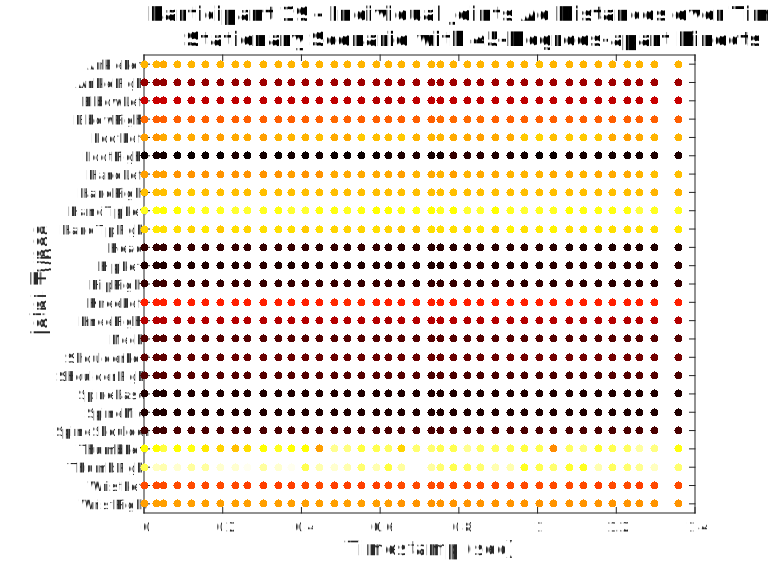
\includegraphics[width=0.666\columnwidth]{Participant_19_Task_Stationary_Kinect_45_Heatmap_hot_dd.pdf} 
    \includegraphics[width=0.666\columnwidth]{Participant_19_Task_Stationary_Kinect_90_Heatmap_hot_dd.pdf} 
  } \\
  \subfloat[Steps]{
    \includegraphics[width=0.666\columnwidth]{Participant_19_Task_Steps_Kinect_Parallel_Heatmap_hot_dd.pdf} 
    \includegraphics[width=0.666\columnwidth]{Participant_19_Task_Steps_Kinect_45_Heatmap_hot_dd.pdf} 
    \includegraphics[width=0.666\columnwidth]{Participant_19_Task_Steps_Kinect_90_Heatmap_hot_dd.pdf} 
  } \\
  \subfloat[Walk]{
    \includegraphics[width=0.666\columnwidth]{Participant_19_Task_Walk_Kinect_Parallel_Heatmap_hot_dd.pdf} 
    \includegraphics[width=0.666\columnwidth]{Participant_19_Task_Walk_Kinect_45_Heatmap_hot_dd.pdf} 
    \includegraphics[width=0.666\columnwidth]{Participant_19_Task_Walk_Kinect_90_Heatmap_hot_dd.pdf} 
  }

  \caption{Average joints distances in the Stationary, Steps, and Walk tasks with Parallel, 45$^{\circ}$ and 90$^{\circ}$ apart Kinects. The figures show heatmaps over different distances values.}

  \label{fig:results_three_joints_over_time}
\end{figure*}

\FloatBarrier
\subsection{Obstacle}

\textbf{show screenshots}

\FloatBarrier
\subsection{Occlusion through interaction}

\textbf{show screenshots}

\FloatBarrier
\subsection{Overall}

\begin{figure*}[!htb]
  \centering

  \includesvg[width=2.0\columnwidth]{Coordinates_All}

  \caption{Overall result}

  \label{fig:results_overall}
\end{figure*}

\begin{table}[!htb]
\centering
\begin{tabularx}{1.0\columnwidth}{||X c c c c||} 
 \hline
 \textbf{Setup} & Avg. $\Delta x$ & Avg. $\Delta y$ & Avg. $\Delta z$ & Avg. $\Delta d$ \\ [0.5ex] 
 \hline\hline
Parallel, Stationery & 1.84 & 3.38 & 7.30 & 4.17 \\
 \hline
 Std. $\Delta x$ & 1.03 & 1.52 & 2.94 & 2.82 \\
 \hline
  & 1.28 & 3.59 & 4.35 & 3.07 \\
 \hline
 Std. $\Delta y$ & 0.49 & 1.50 & 2.15 & 1.60 \\
 \hline
  & 2.08 & 3.17 & 5.1917 & 3.48 \\
 \hline
 Std. $\Delta z$ & 0.89 & 1.45 & 1.84 & 1.58 \\
 \hline
  & 3.52 & 6.95 & 11.39 & 7.29 \\
 \hline
 Std. $\Delta d$ & 1.33 & 2.67 & 4.45 & 3.95 \\
 \hline
\end{tabularx}
\caption{Average coordinates distances in the Walk task for three different Kinect placements}
\label{table:overall_coordinates_values}
\end{table}
